\documentclass[12pt, letterpaper]{report}
\usepackage[utf8]{inputenc}
\usepackage{amsmath}
\usepackage{changepage}% http://ctan.org/pkg/changepage
\newcommand\tab[1][1cm]{\hspace*{#1}}
\usepackage{graphicx}


\title{CS M148 Homework 1}
\author{Hanna Co}
\date{Due: January 28, 2021}

\begin{document}
\maketitle
\noindent {\large{\textbf{1 \tab Data and Bias} }} \\\\
\indent (a) Undercoverage bias, because we are only getting responses from those with Twitter. Convenience sample, because our sample is not random.
\\\\
\indent (b) It was discriminating against women because not a lot of Amazon employees are women, so it may have been biased against women. Dropping gender may not have been enough because it may have developed a bias agains universities, organizations, or opportunities available only to women, or because of traditionally female names.

\newpage
\noindent {\large{\textbf{2 \tab KNN Regression} }} \\\\
\indent (a) 1-NN:\\
\tab $x = 0 \Rightarrow y = 1$\\
\tab $x = 1 \Rightarrow y = 0$\\
\tab $x = 2 \Rightarrow y = 5$\\
\tab $x = 3 \Rightarrow y = 2$\\
\tab $x = 4 \Rightarrow y = 5$\\
\indent 3-NN:\\
\tab $x = 0 \Rightarrow y = \frac{1}{3}(0+1+5) = 2$\\
\tab $x = 1 \Rightarrow y = \frac{1}{3}(0+1+5) = 2$\\
\tab $x = 2 \Rightarrow y = \frac{1}{3}(0+5+2) = \frac{7}{3}$\\
\tab $x = 3 \Rightarrow y = \frac{1}{3}(5+2+5) = 4$\\
\tab $x = 4 \Rightarrow y = \frac{1}{3}(5+2+5) = 4$\\
\indent 5-NN:\\
\tab $x = 0 \Rightarrow y = \frac{1}{5}(1+0+5+2+5) = 2.6$\\
\tab $x = 1 \Rightarrow  y = \frac{1}{5}(1+0+5+2+5) = 2.6$\\
\tab $x = 2 \Rightarrow y = \frac{1}{5}(1+0+5+2+5) = 2.6$\\
\tab $x = 3 \Rightarrow y = \frac{1}{5}(1+0+5+2+5) = 2.6$\\
\tab $x = 4 \Rightarrow y = \frac{1}{5}(1+0+5+2+5) = 2.6$\\
\begin{figure}[h!]
  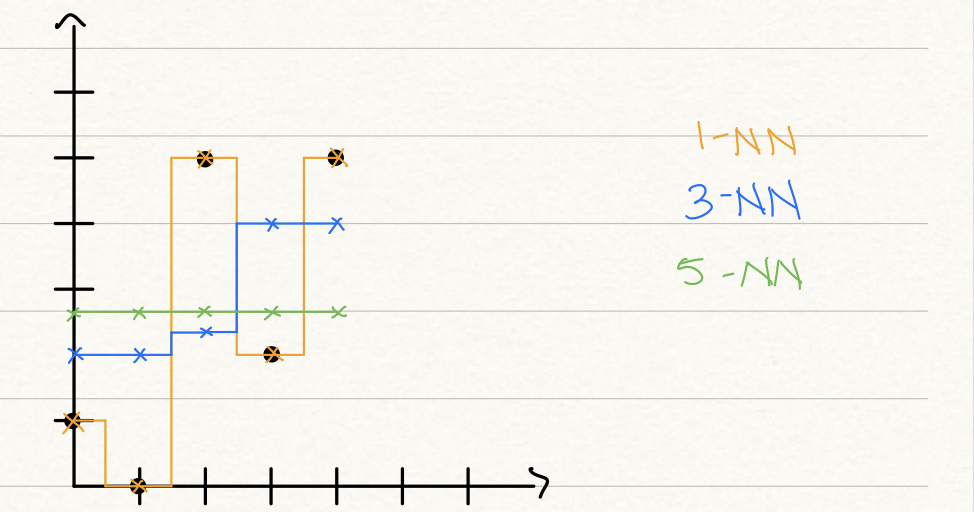
\includegraphics[width=\linewidth]{./images/neighbor_graph.jpeg}
\end{figure}
\\\\
\indent (b)\\
\tab $K = 1: (0.5, 0) (1.5, 0) (2.5, 2) (3.5, 2) MSE = 3.75$\\
\tab $K = 2: (0.5, 0.5) (1.5, 2.5) (2.5, 3.5) (3.5, 3.5) MSE = 0.25$\\
\tab $K = 3: (0.5, 2) (1.5, 2) (2.5, \frac{7}{3}) (3.5, 4) MSE = 1.44$\\
\tab $K = 4: (0.5, 2) (1.5, 2) (2.5, 3) (3.5, 3) MSE = 0.75$\\
\tab $K = 5: (0.5, 2.6) (1.5, 2.6) (2.5, 2.6) (3.5, 2.6) MSE = 1.21$\\
Based off MSE, $K = 2$ has the lowest MSE, thus $K = 2$ is the best.
\\\\
\indent (c) $R^2 = 1 - \frac{\sum_{i=1}^{n} (\hat{y_i} - y_1)^2}{\sum_{i=1}^{n} (\bar{y_i} - y_1)^2}$\\
When $K = 1$ on the training data, we have $R^2 = 1$, which means our model is perfect. However, when applying this model to our test data sets, it may not be the best, because it's "too precise" and overfitted to the training set, and it may not perform well for the test data.

\newpage
\noindent {\large{\textbf{3 \tab Linear Regression} }} \\\\
\indent (a)$\mathcal{L}(\beta_0, \beta_1) = \frac{1}{n}\sum_{i=1}^{n} (y_i - [\beta_0 + \beta_1x_i])^2$\\\\
\tab$\frac{\partial\mathcal{L}}{\partial\beta_0} = \frac{1}{n}\sum_{i=1}^{n} -2(y_i - [\beta_0 + \beta_1x_i])$\\\\
\tab$\frac{1}{n}\sum_{i=1}^{n} -2(y_i - [\beta_0 + \beta_1x_i]) = 0$\\\\
\tab$\frac{-2}{n}[(-n\beta_0) + \sum_{i=1}^{n} y_i - \beta_1 \sum_{i=1}^{n} x_i] = 0$\\\\
\tab$\frac{-2}{n}[(-n\beta_0) + \sum_{i=1}^{n} y_i - \beta_1 \sum_{i=1}^{n} x_i] = 0$\\\\
\tab$n\beta_0 = \sum_{i=1}^{n} y_i - \beta_1x_i$\\\\
\tab$\beta_0 = \frac{1}{n}\sum_{i=1}^{n} y_i - \beta_1x_i$\\\\
\tab$\beta_0 = \bar{y} - \beta_1\bar{x}$\\\\
\\
\tab$\frac{\partial\mathcal{L}}{\partial\beta_1} = \frac{1}{n}\sum_{i=1}^{n} -2x_i(y_i - [\beta_0 + \beta_1x_i])$\\\\
\tab$\frac{1}{n}\sum_{i=1}^{n} -2x_i(y_i - [\beta_0 + \beta_1x_i]) = 0$\\\\
\tab$\frac{-2}{n}\sum_{i=1}^{n} x_i(y_i - \beta_0 - \beta_1x_i) = 0$\\\\
\tab$\sum_{i=1}^{n} x_iy_i - x_i\beta_0 - \beta_1 x^2_i) = 0$\\\\
\tab$\sum_{i=1}^{n} x_iy_i - \beta_0\sum_{i=1}^{n}x_i  = \beta_1 \sum_{i=1}^{n}x^2_i$\\\\
\tab$\sum_{i=1}^{n} x_iy_i - (\bar{y}-\beta_1\bar{x})\sum_{i=1}^{n}x_i  = \beta_1 \sum_{i=1}^{n}x^2_i$\\\\
\tab$\sum_{i=1}^{n} x_iy_i - \bar{y}\sum_{i=1}^{n}x_i + \beta_1\bar{x}\sum_{i=1}^{n}x_i  = \beta_1 \sum_{i=1}^{n}x^2_i$\\\\
\tab$\sum_{i=1}^{n} x_iy_i - \frac{1}{n}\sum_{i=1}^{n}y_i\sum_{i=1}^{n}x_i = \beta_1 \sum_{i=1}^{n}x^2_i - \beta_1\frac{1}{n}\sum_{i=1}^{n}x_i\sum_{i=1}^{n}x_i $\\\\
\tab$\sum_{i=1}^{n} x_iy_i - \frac{1}{n}(n\bar{y})(n\bar{x}) = \beta_1 (\sum_{i=1}^{n}x^2_i - \frac{1}{n}(\sum_{i=1}^{n}x_i)^2)$\\\\
\tab$\sum_{i=1}^{n} x_iy_i - n\bar{y}\bar{x} = \beta_1 (\sum_{i=1}^{n}x^2_i - \frac{1}{n}(n\bar{x})^2)$\\\\
\tab$\sum_{i=1}^{n} x_iy_i - n\bar{y}\bar{x} = \beta_1 (\sum_{i=1}^{n}x^2_i - n\bar{x}^2)$\\\\
\tab$\sum_{i=1}^{n} (x_i-\bar{x})(y_i-\bar{y}) = \beta_1 (\sum_{i=1}^{n}(x_i - \bar{x})^2)$\\\\
\tab$\beta_1 = \frac{\sum_{i=1}^{n} (x_i-\bar{x})(y_i-\bar{y})}{\sum_{i=1}^{n}(x_i - \bar{x})^2}$\\\\
\\\\
\indent (b) $Y = \beta_0 \Rightarrow \mathcal{L}(\beta_0) = \frac{1}{n}\sum_{i=1}^{n}(y_i - \beta_0)^2$\\\\
\tab MSE = $\frac{1}{n}\sum_{i=1}^{n}(y_i - [\beta_0 + \beta_1x_i])^2$\\\\
\tab$\frac{\partial\mathcal{L}}{\partial\beta_0} = \frac{1}{n}\sum_{i=1}^{n}2(y_i - \beta_0)(-1)$\\\\
\tab$\frac{1}{n}\sum_{i=1}^{n}-2(y_i - \beta_0) = 0$\\\\
\tab$\sum_{i=1}^{n}y_i - \sum_{i=1}^{n}\beta_0 = 0$\\\\
\tab$n\bar{y} = n\beta_0$\\\\
\tab $\beta_0 = \bar{y} \Rightarrow $ the optimal value for $\beta_0$ is $\bar{y}$\\\\
\\
\tab MAE = $\frac{1}{n}\sum_{i=1}^{n} \lvert y_i - \beta_0 \rvert$\\\\
\tab$\frac{\partial\mathcal{L}}{\partial\beta_0} = \frac{1}{n}\sum_{i=1}^{n}\frac{y_i-\beta_0}{\lvert y_i-\beta_0\rvert}$\\\\
\tab$\frac{1}{n}\sum_{i=1}^{n}\frac{y_i-\beta_0}{\lvert y_i-\beta_0\rvert} = 0$\\\\
\tab$\sum_{i=1}^{n}sign(y_i-\beta_0) = 0$\\\\
The optimal value of $\beta_0$ is when there are an equal number of $y$ values greater than $\beta_0$ and less than $\beta_0$, which is, be definition, the median.

\newpage
\noindent {\large{\textbf{4 \tab Linear Regression: goodness of fit \& Interpretation} }} \\\\
1\\
\indent (a) $\beta_0 = \bar{y} - \beta_1\bar{x}$\tab\tab $\beta_1 = \frac{\sum_{i=1}^{n}x_iy_i-\bar{y}x_i}{\sum_{i=1}^{n}x^2_i - \bar{x}x_i}$\\
\indent$\bar{y} = 111,200,000$\\
\indent$\bar{x} = 1900$\\\\
\indent$\sum_{i=1}^{n}x_iy_i-\bar{y}x_i = [(1800)(5,000,000) - (111,200,000)(1800)] + [(1850)(23,000,000) - (111,200,000)(1850)] + [(1900)(76,000,000) - (111,200,000)(1900)] + [(1950)(161,000,000) - (111,200,000)(1950)] + [(2000)(291,000,000) - (111,200,000)(2000)]$\\
\indent$= -191,160,000,000 - 16,317,000,000 - 66,880,000,000 + 97,110,000,000 + 359,600,000,000$\\
\indent$= 35,500,000,000$\\
\indent$\sum_{i=1}^{n}x^2_i - \bar{x}x_i = [1800^2 - (1800)(1900)] + [1850^2 - (1850)(1900)] + [1900^2 - (1900)(1900)] + [1950^2 - (1950)(1900)] + [2000^2 - (2000)(1900)]$\\
\indent$-180,000 - 92,500 + 0 + 97,500 + 200,000$\\
\indent$= 25,000$\\
\indent$\beta_1 = \frac{35,500,000,000}{25,000} = 1,420,000$\\
\indent$\beta_0 = 111,200,000-(\beta_1)(1900) = -2,586,800,000$
\\\\
\indent (b)$R^2 = 1 - \frac{\sum_{i=1}^{n} (\hat{y_i} - y_1)^2}{\sum_{i=1}^{n} (\bar{y_i} - y_1)^2}$\tab\tab $\hat{y} = \beta_0 + \beta_1x_i$\\
\indent$\sum_{i=1}^{n} (\hat{y_i} - y_1)^2 = (-30,800,000 - 5,000,000)^2 + (40,200,000 - 23,000,000)^2 + (111,200,000 - 76,000,000)^2 + (182,200,000 - 161,000,000)^2 + (253,200,000 - 291,000,000)^2$\\
\indent$= 4.6948 \times 10^{15}$\\
\indent$\sum_{i=1}^{n} (\bar{y_i} - y_1)^2 = (111,200,000 - 5,000,000)^2 + (111,200,000 - 23,000,000)^2 + (111,200,000 - 76,000,000)^2 + (111,200,000 - 161,000,000)^2 + (111,200,000 - 291,000,000)^2 $\\
\indent$= 5.51048 \times 10^{16}$\\
\indent$R^2 = 1 - \frac{4.6948 \times 10^{15}}{5.51048 \times 10^{16}} = 1 - 0.0852 = 0.915$\\
\indent We have $R^2 = 0.915$, which is very close to 1, indicating that our model is very good.\\\\
\\\\\\
\indent (c)
\begin{figure}[h!]
  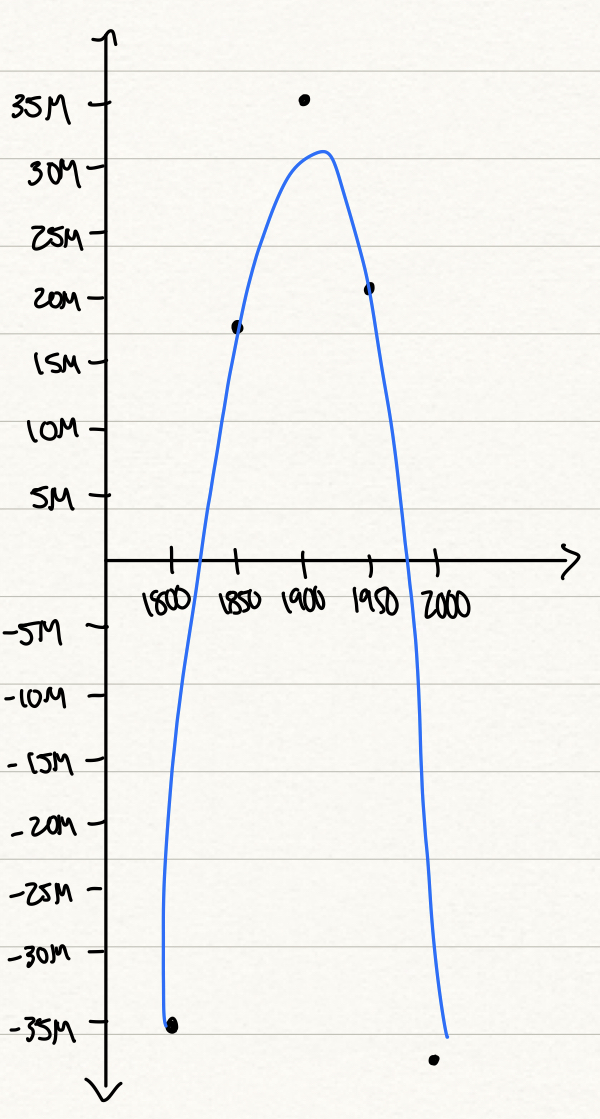
\includegraphics[scale=0.25]{./images/residual_graph.jpeg}
\end{figure}\\
From the residual graph, I conclude that the population growth from 1800-2000 is not necessarily linear.
\\\\
2 While we observe a fairly strong negative correlation between wine consumption and heart disease (as indicated by $R^2 = 71.0\%$), we cannot conclude that drinking more wine reduces the risk of heart disease, because correlation does not equal causation.\\
\\
3\\
\indent (a) (i) $\beta_0 = -30.83, \beta_1 = 1.47$\\
\tab (ii) $\beta_0 = 113.98, \beta_1 = -0.681$\\
\\
\indent (b)(i) $R^2 = 0.658$\\
\tab (ii) $R^2 = 0.639$\\
It seems that, on average, as the percentage of sunny days increases, less pesticide is used. It also appears that, one average, as pesticide use increases, the amount of diseased crops increases. It may appear that the disease rate increases as more pesticide is used, but it could be possible that the increased pesticide use is in response to disease.
\\\\
4\\
\indent (a) $\beta_0 = 5.006, \beta_1 = 0.1$
\\\\
\indent (b) $R^2 = 0.243$. This does not show a strong linear relation between x and y.
\\\\
\indent (c) We have a p-value of $2.438 \times 10^{-64}$. $2.438 \times 10^{-64} < 0.05$, so we reject the null hypothesis.
\\\\
\indent (d) $\beta_1 \pm 2 \times SE(\beta_1)$ gives us a confidence interval of $[0.0886, 0.111]$, which suggests that our $\beta_1$ value is not meaningfully different from 0.
\\\\
\indent (e) The contradiction is that in (c), we reject the null hypothesis that $\beta_1 = 0$, but in (d), we conclude that since our $\beta_1 \leq 1$, it is not meaningfully different from 0. This contradiction likely comes from the large range of y values in our dataset. In the future, it may be better to do some data cleaning to ensure better results.
\\\\
5\\
\indent (a) $R^2 = 0.75$, indicating that there is a strong linear relationship between the duration of the last eruption and the time until the next eruption.
\\\\
\indent (b) $\hat{y} = 60.383$, and we have a prediction interval of $[57.784, 62.983]$. We can be 95\% confident that if we observe an eruption that is 3 minutes long, the next eruption will happen in $[57.784, 62.983]$ minutes.
\\\\
\indent (c) Given only 60 minutes, I would be able to make a decision, given that 60 minutes falls within the prediction interval.
\\\\

\newpage
\noindent {\large{\textbf{5 \tab Interpretation of Coefficients in Linear Regression} }} \\\\
\indent (a) One way to model this would be to have plant type be a categorical variable. $X_1$ is a numerical variable representing how much sunlight a plant receives. $X_2$ and $X_3$ are categorical variables for plant type: if we have plant type 1, $X_2 = 0$ and $X_3 = 0$. If we have plant type 2, then $X_2 = 1$ and $X_3 = 0$. Otherwise, we have plant type 3, where $X_2 = 0$ and $X_3 = 1$.\\\\
Our linear model is $Y = \beta_1X_1 + \beta_2X_2 + \beta_3X_3 + \beta_0$. $\beta_0$ represents the average growth for plant type 1 when exposed to no sun, $\beta_1$ represents the average growth of all plant types when exposed to sun. $\beta_2$ is the average difference in plant growth between plant types 1 and 2, and $\beta_3$ is the average differece in plant growth between plant types 1 and 3.
\\\\
\indent (b) To test whether the independent variables have a significant correlation with our dependent variables $Y$, we can calculate t-test values for $\beta_1, \beta_2, \beta_3$. We can then get corresponding p-values. If a p-value is small, then we reject the null hypothesis that there is no relationship between $Y$ and the corresponding predictor variable.

\newpage
\noindent {\large{\textbf{6 \tab Model Evaluation} }} \\\\
With random sampling, only 5\% of data points have $y=0$, so the issue is that the random sample may not accurately represent the dataset. To address this, we can take a stratified sample, where 5\% of our sample contains points where $y=0$, and the other 95\% contain points where $y=1$. This way, our sample better represents the population.
\end{document}